%% intro
Surface normal inference from a single view deals with the task of object surface orientation estimation. It has many practical applications, such as augmented reality and robotics. 




%%%%%%%%%%%%%%%%%%% talk about the reason of this thesis %%%%%%%%%%%%%%%%%%

%% standard method for normal inference is insufficient, input is sparse, not robust enough
Standard methods compute normals from point cloud using neighboring information in image space or use Shape from Shading. However, the point clouds data provided by Kinect or similar RGB-D, LiDAR sensors are only semi-dense. As shown in Figure \ref{fig:depth_map_with_noise}. If map these normals to polygon mesh, that is not good at all. 

%% add noise image
\begin{figure}[!h]
	\centering
	\begin{tikzpicture}
		\node[inner sep=0pt] (depthmap) at (0,0)
		{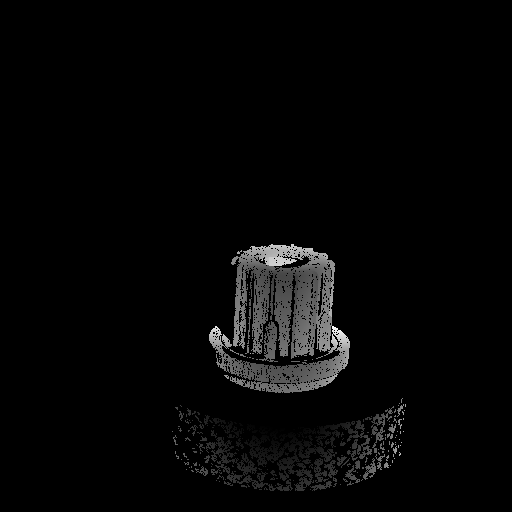
\includegraphics[width=.5\textwidth]{./pic/00028.depth0.png}};
	\end{tikzpicture}
	\caption{A depth map captured via infrared sensors. The missing pixels distributed almost all of the image.}
	\label{fig:depth_map_with_noise}
\end{figure}

Standard methods derives normal from each point and its neighborhoods' positions. It dependents on chosen neighbor size. There are two main drawbacks. First, if neighbor size is too small, it has larger noise sensitive, if it is too large, the output will too smooth and not crispy. Second, it is not robust with noise.  Errors may occur in regions with inter-reflections, where we have errors in the 3D measurement. On the other side, it is also weak with missing pixel handling, which is a common issue in depth maps.

%% add noise image
\begin{figure}[!h]
	\centering
	\begin{tikzpicture}	
		\node[inner sep=0pt] (normal) at (8,0)
		{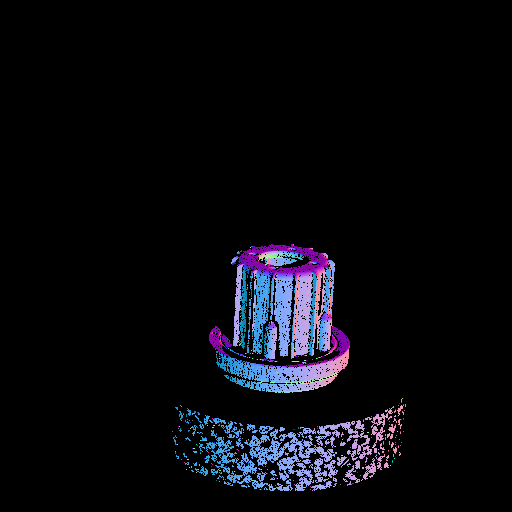
\includegraphics[width=.5\textwidth]{./pic/00028.normal0.png}};
	\end{tikzpicture}
	\caption{Semi-dense Normal Map calculated from depth map using standard method}
	\label{fig:standard_normal_inference}
\end{figure}

%% there exists space for improvment 
Although the depth image is incomplete, the depth sensor usually able to capture grayscale texture image, which are typically fully dense due to their passive nature. Furthermore, if the texture image is already illuminated by strong directional light of a video projector, whose position is known, then there should exist theoretical relations between light direction, normal direction, and grayscale image . Thus the normal can be inferenced better using the given image information and depth map. 

%%%%%%%%%%%%%%%%%%% talk about the chanllege of this task %%%%%%%%%%%%%%%%%%
Both depth and grayscale image are initially relevant to the machine learning algorithms. Based grayscale image and corresponding semi-dense depth map, a CNN model can be designed to inference the normal map, which gives more density and robust comparing to standard algorithm. However, the missing pixels in depth map can be distributed around the whole image, some of the image regions leave complete empty holes. This situation imposes further processing for the missing regions and some other challenges on the machine learning methods. 
In this thesis, we found a solution for the problems mentioned above.

%% CNN based methods
The deep convolutional neural network is typically used for image classification, which achieved great success in last several years. \cite{yolov3}, \cite{efficientDet}. 
%% talk about the reason we need new type of network architecture
These kinds of network architecture takes a single image as input which usually employed for classification problems. The image is usually convoluted with convolutional layer and downsampling with pooling layers. The outputs of the network consists of a single value to represent the ID of corresponding class \cite{efficientDet}, or with set of values to represent the position of bounding boxes.\cite{yolov3}.


However, in many other vision tasks, the output is demanded as an image, instead of predicting one or several classes of the input, but the classes of each pixel are predicted, like image segmentation\cite{unet}. In this case, the traditional network architecture is not suitable anymore.

%% improved normal inference figure
\begin{figure}[!h]
	\centering
	\begin{tikzpicture}
		
		\node[inner sep=0pt] (image) at (0,0)
		{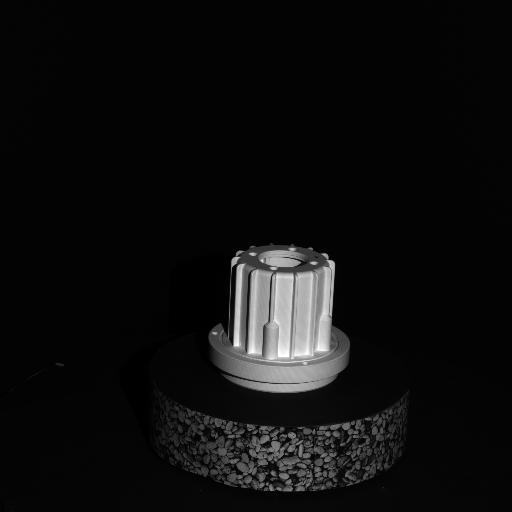
\includegraphics[width=.2\textwidth]{./pic/00028.image0.png}};
		
		\node[text width=1cm] at (2,0) {$ + $};
		
		\node[inner sep=0pt] (depthmap) at (3.3,0)
		{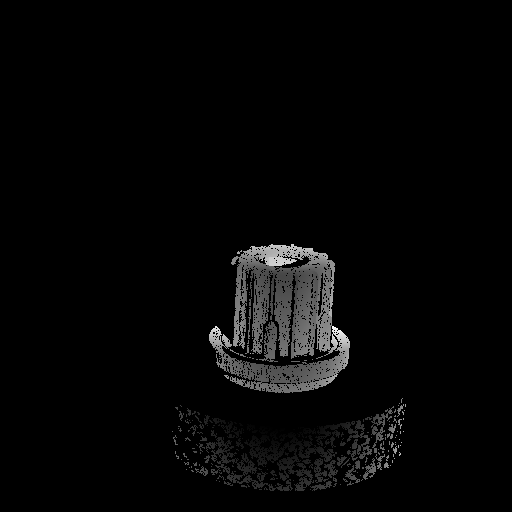
\includegraphics[width=.2\textwidth]{./pic/00028.depth0.png}};
		\node[text width=1cm] at (8,0) {$ ? $};
		
		\path [line] (5,0) -- node [text width=1cm,midway,above ] {CNN} (6,0);
		
	\end{tikzpicture}
	\caption{Left: Grayscale Image, Middle: Depth Map}
	\label{fig:improved_normal_inference}
\end{figure}


In this thesis, we proposed a novel deep learning architecture for surface normal inference. 

By applying our approach to the task of normal inference, a custom dataset is created from Unity using 3D models. The trained Normal models achieve a remarkably better prediction accuracy at a low computational cost comparing to the standard approaches for semi-dense point clouds. 




















